\section{Finding  - Possible determination of OpenSSL version}
\hrule\begin{table}[htb]
    \renewcommand{\arraystretch}{1.5}
    \begin{tabular*}{\textwidth}{|>{\columncolor{gray!15}}p{3cm}|p{17.2cm}|}
    \textbf{Finding} & \textbf{Possible determination of OpenSSH version }\\
    Risk& Informational\\
    Category& Information Disclosure\\
    Impact& An attacker is able to see the OpenSSL version of the service running on port 22\\\\
    Description& As shown in the graphic below the output of an nmap scan disclosed the version of the OpenSSH server.
    \newline
    \newline
    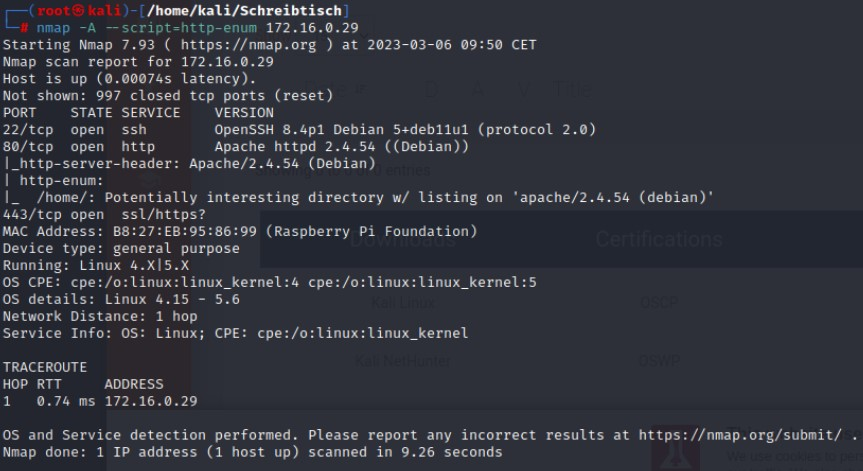
\includegraphics[width=0.85\textwidth]{http_vulnerbility.jpg}
	\\ 
	&\\
	&\\
    Recommendation& Edit the OpenSSH server configuration and add the following line at the end: \newline ''VersionAddendum none''\\    
    \\\\\\\\\\\\
    \end{tabular*}
    \end{table}